\documentclass[10pt]{article}
\usepackage{tmlr}
% Short version of BELLROUTE_TMLR.tex. Same data, numbers, and figures; condensed prose.

\usepackage[T1]{fontenc}
\usepackage[utf8]{inputenc}
\usepackage{amsmath,amssymb,amsthm}
\usepackage{booktabs}
\usepackage{tabularx}
\usepackage{array}
\usepackage{graphicx}
\usepackage{xcolor}
\usepackage{enumitem}
\usepackage{microtype}
\usepackage{float}
\usepackage{hyperref}
\usepackage{url}
\usepackage[nameinlink,capitalise]{cleveref}

\hypersetup{
  pdftitle={Beating Greedy Is Not Enough: A Preregistered Benchmark for Budgeted Allocation of Certified Entanglement},
  pdfauthor={Anonymous},
  colorlinks=true, linkcolor=blue!50!black, citecolor=blue!50!black, urlcolor=blue!50!black,
}

% Generated by make_numbers.py from the Stage 29 audit; do not edit by hand.
\newcommand{\ablBinary}{0.1881}
\newcommand{\ablDropBinary}{41}
\newcommand{\ablDropNoBudget}{33}
\newcommand{\ablDropNoHorizon}{56}
\newcommand{\ablDropShuffled}{49}
\newcommand{\ablNoBudget}{0.2165}
\newcommand{\ablNoHorizon}{0.1415}
\newcommand{\ablShuffled}{0.1639}
\newcommand{\catCmpClassical}{0.000}
\newcommand{\catCmpDQN}{0.544}
\newcommand{\catCmpFuture}{0.601}
\newcommand{\catCmpGreedy}{0.323}
\newcommand{\catCmpMessage}{10.191}
\newcommand{\catCmpOnline}{0.579}
\newcommand{\catCmpPPO}{0.486}
\newcommand{\catCmpRandom}{0.173}
\newcommand{\catCmpStatic}{0.249}
\newcommand{\catPathClassical}{0.000}
\newcommand{\catPathDQN}{0.611}
\newcommand{\catPathFuture}{0.741}
\newcommand{\catPathGreedy}{0.308}
\newcommand{\catPathMessage}{12.121}
\newcommand{\catPathOnline}{0.702}
\newcommand{\catPathPPO}{0.623}
\newcommand{\catPathRandom}{0.197}
\newcommand{\catPathStatic}{0.224}
\newcommand{\catRingClassical}{0.000}
\newcommand{\catRingDQN}{0.503}
\newcommand{\catRingFuture}{0.626}
\newcommand{\catRingGreedy}{0.300}
\newcommand{\catRingMessage}{15.551}
\newcommand{\catRingOnline}{0.590}
\newcommand{\catRingPPO}{0.527}
\newcommand{\catRingRandom}{0.206}
\newcommand{\catRingStatic}{0.186}
\newcommand{\catSparseClassical}{0.000}
\newcommand{\catSparseDQN}{1.167}
\newcommand{\catSparseFuture}{1.403}
\newcommand{\catSparseGreedy}{0.743}
\newcommand{\catSparseMessage}{42.270}
\newcommand{\catSparseOnline}{1.353}
\newcommand{\catSparsePPO}{1.143}
\newcommand{\catSparseRandom}{0.329}
\newcommand{\catSparseStatic}{0.283}
\newcommand{\develDDQN}{0.3209}
\newcommand{\develDDQNMinusPPO}{-0.0039}
\newcommand{\develDQN}{0.3235}
\newcommand{\develPPO}{0.3247}
\newcommand{\develRPPO}{0.3047}
\newcommand{\diffCmp}{-0.059}
\newcommand{\diffPath}{+0.011}
\newcommand{\diffRing}{+0.024}
\newcommand{\diffSparse}{-0.024}
\newcommand{\dqnMinusGreedy}{+0.288}
\newcommand{\dqnSeedsAboveGreedy}{12}
\newcommand{\eqMargin}{0.0403}
\newcommand{\fracCmpDQN}{94.0}
\newcommand{\fracCmpGreedy}{55.8}
\newcommand{\fracCmpPPO}{83.9}
\newcommand{\fracDQN}{87.7}
\newcommand{\fracFuture}{104.5}
\newcommand{\fracGreedy}{51.9}
\newcommand{\fracPPO}{86.2}
\newcommand{\fracPathDQN}{87.0}
\newcommand{\fracPathGreedy}{43.8}
\newcommand{\fracPathPPO}{88.6}
\newcommand{\fracRingDQN}{85.3}
\newcommand{\fracRingGreedy}{50.8}
\newcommand{\fracRingPPO}{89.4}
\newcommand{\fracSparseDQN}{86.3}
\newcommand{\fracSparseGreedy}{54.9}
\newcommand{\fracSparsePPO}{84.5}
\newcommand{\holmpCmp}{1.000}
\newcommand{\holmpPath}{0.096}
\newcommand{\holmpRing}{0.068}
\newcommand{\holmpSparse}{1.000}
\newcommand{\meanClassical}{0.0000}
\newcommand{\meanDQN}{0.7065}
\newcommand{\meanFuture}{0.8426}
\newcommand{\meanGreedy}{0.4183}
\newcommand{\meanMessage}{20.0331}
\newcommand{\meanOnline}{0.8060}
\newcommand{\meanPPO}{0.6946}
\newcommand{\meanRandom}{0.2263}
\newcommand{\meanStatic}{0.2354}
\newcommand{\noiseHerFive}{0.3298}
\newcommand{\noiseHerSevenFive}{0.5134}
\newcommand{\noiseIdealHundred}{0.6892}
\newcommand{\noiseVisEight}{0.0000}
\newcommand{\noiseVisSix}{0.0000}
\newcommand{\onlineMean}{0.8060}
\newcommand{\paramsDQN}{9{,}153}
\newcommand{\paramsPPO}{18{,}306}
\newcommand{\phFracDQN}{86.0}
\newcommand{\phFracGreedy}{53.7}
\newcommand{\phFracPPO}{86.0}
\newcommand{\phMargin}{0.0486}
\newcommand{\phPPOMinusDqn}{+0.0000}
\newcommand{\phPPOMinusDqnHiNinety}{+0.0159}
\newcommand{\phPPOMinusDqnLoNinety}{-0.0168}
\newcommand{\phPPOMinusGreedy}{+0.314}
\newcommand{\phPPOMinusGreedyHi}{+0.322}
\newcommand{\phPPOMinusGreedyLo}{+0.305}
\newcommand{\posOppEight}{0.0}
\newcommand{\posOppIdeal}{74.9}
\newcommand{\posOppNine}{11.8}
\newcommand{\posOppNineFive}{52.5}
\newcommand{\ppoDistinctSeedValues}{8}
\newcommand{\ppoMinusDqn}{-0.0118}
\newcommand{\ppoMinusDqnHiNinety}{-0.0011}
\newcommand{\ppoMinusDqnHiNinetyFive}{+0.0004}
\newcommand{\ppoMinusDqnLoNinety}{-0.0240}
\newcommand{\ppoMinusDqnLoNinetyFive}{-0.0265}
\newcommand{\ppoMinusGreedy}{+0.276}
\newcommand{\ppoMinusGreedyHi}{+0.283}
\newcommand{\ppoMinusGreedyLo}{+0.269}
\newcommand{\ppoSeedsAboveDqn}{5}
\newcommand{\ppoSeedsAboveGreedy}{12}
\newcommand{\progCPU}{4.79}
\newcommand{\progDecisions}{3{,}360{,}912}
\newcommand{\progUpdates}{683{,}090}
\newcommand{\progWallHours}{4.79}
\newcommand{\ratioHerFive}{0.479}
\newcommand{\ratioHerSevenFive}{0.745}
\newcommand{\rawpCmp}{1.000}
\newcommand{\rawpPath}{0.032}
\newcommand{\rawpRing}{0.017}
\newcommand{\rawpSparse}{0.935}
\newcommand{\resAllocUpdates}{351{,}756}
\newcommand{\resBaseline}{148{,}000}
\newcommand{\resCPU}{2.31}
\newcommand{\resCertUpdates}{204{,}800}
\newcommand{\resCircuits}{1{,}843{,}200}
\newcommand{\resDecisions}{2{,}081{,}152}
\newcommand{\resDqnTrain}{446}
\newcommand{\resEvalPrimary}{888{,}000}
\newcommand{\resEvalSecondary}{355{,}200}
\newcommand{\resPpoTrain}{175}
\newcommand{\resTrainDecisions}{689{,}952}
\newcommand{\resWall}{8{,}324}
\newcommand{\resWallHours}{2.31}
\newcommand{\sOneBer}{0.5064}
\newcommand{\sOneDP}{0.5712}
\newcommand{\sOneDiff}{+0.1980}
\newcommand{\sOneDiffHi}{+0.2043}
\newcommand{\sOneDiffLo}{+0.1914}
\newcommand{\sOneFrac}{88.66}
\newcommand{\sOneFracLo}{87.68}
\newcommand{\sOneFuture}{0.5833}
\newcommand{\sOneGreedy}{0.3084}
\newcommand{\sOneRandom}{0.2268}
\newcommand{\sOneSeedsAbove}{16}
\newcommand{\sOneStatic}{0.2248}
\newcommand{\testOpportunities}{255}
\newcommand{\testPositiveTypes}{12}
\newcommand{\testTypes}{16}
\newcommand{\thrNonTestMedian}{0.9824}
\newcommand{\thrNonTestMin}{0.8511}
\newcommand{\thrTestMean}{0.9562}
\newcommand{\thrTestMedian}{0.9620}
\newcommand{\thrTestMin}{0.8491}
\newcommand{\validDDQNHerFive}{0.1596}
\newcommand{\validDDQNHerNine}{0.2924}
\newcommand{\validDDQNHerSevenFive}{0.2463}
\newcommand{\validDDQNIdeal}{0.3205}
\newcommand{\validDDQNVisEight}{0.0000}
\newcommand{\validDDQNVisNine}{0.0139}
\newcommand{\validDDQNVisSeven}{0.0000}
\newcommand{\validDDQNVisSix}{0.0000}
\newcommand{\validDQNHerFive}{0.1593}
\newcommand{\validDQNHerNine}{0.2946}
\newcommand{\validDQNHerSevenFive}{0.2485}
\newcommand{\validDQNIdeal}{0.3220}
\newcommand{\validDQNVisEight}{0.0000}
\newcommand{\validDQNVisNine}{0.0101}
\newcommand{\validDQNVisSeven}{0.0000}
\newcommand{\validDQNVisSix}{0.0000}
\newcommand{\validPPOHerFive}{0.1635}
\newcommand{\validPPOHerNine}{0.2980}
\newcommand{\validPPOHerSevenFive}{0.2526}
\newcommand{\validPPOIdeal}{0.3273}
\newcommand{\validPPOVisEight}{0.0000}
\newcommand{\validPPOVisNine}{0.0000}
\newcommand{\validPPOVisSeven}{0.0000}
\newcommand{\validPPOVisSix}{0.0000}
\newcommand{\validPosOppIdeal}{54.8}
\newcommand{\validPosOppNine}{9.52}
\newcommand{\validRPPOHerFive}{0.1620}
\newcommand{\validRPPOHerNine}{0.2938}
\newcommand{\validRPPOHerSevenFive}{0.2480}
\newcommand{\validRPPOIdeal}{0.3225}
\newcommand{\validRPPOVisEight}{0.0000}
\newcommand{\validRPPOVisNine}{0.0000}
\newcommand{\validRPPOVisSeven}{0.0000}
\newcommand{\validRPPOVisSix}{0.0000}
\newcommand{\winsCmp}{0}
\newcommand{\winsPath}{9}
\newcommand{\winsRing}{11}
\newcommand{\winsSparse}{4}

% Generated by make_tmlr_assets.py from the Stage-30 to 34 bundles; do not edit by hand.
\newcommand{\bpAlpha}{0.75}
\newcommand{\bpConfigs}{35}
\newcommand{\bpFrac}{97.2}
\newcommand{\bpFracFresh}{96.6}
\newcommand{\bpMean}{0.7836}
\newcommand{\bpPrior}{80}
\newcommand{\bpValMean}{0.3534}
\newcommand{\catCmpBp}{0.562}
\newcommand{\catCmpCeZero}{0.578}
\newcommand{\catPathBp}{0.696}
\newcommand{\catPathCeZero}{0.702}
\newcommand{\catRingBp}{0.577}
\newcommand{\catRingCeZero}{0.589}
\newcommand{\catSparseBp}{1.300}
\newcommand{\catSparseCeZero}{1.352}
\newcommand{\ceConfigs}{26}
\newcommand{\ceFracMax}{100.0}
\newcommand{\ceFracMin}{99.6}
\newcommand{\ceZeroFrac}{99.9}
\newcommand{\ceZeroMean}{0.8052}
\newcommand{\cfAlpha}{0.75}
\newcommand{\cfCPU}{6.7}
\newcommand{\cfDecision}{bid price superior}
\newcommand{\cfDqnDecision}{bid price superior}
\newcommand{\cfDqnMinusBp}{-0.180}
\newcommand{\cfDqnMinusBpHi}{-0.157}
\newcommand{\cfDqnMinusBpLo}{-0.204}
\newcommand{\cfDqnMinusBpWins}{0}
\newcommand{\cfDqnMinusGreedy}{+0.308}
\newcommand{\cfDqnMinusGreedyHi}{+0.331}
\newcommand{\cfDqnMinusGreedyLo}{+0.285}
\newcommand{\cfDqnMinusGreedyWins}{12}
\newcommand{\cfEqMargin}{0.044}
\newcommand{\cfForesight}{4.7}
\newcommand{\cfFracBp}{98.5}
\newcommand{\cfFracCe}{99.9}
\newcommand{\cfFracDqn}{77.9}
\newcommand{\cfFracGreedy}{42.6}
\newcommand{\cfFracMaxBp}{98.7}
\newcommand{\cfFracMaxCe}{100.1}
\newcommand{\cfFracMaxDqn}{93.9}
\newcommand{\cfFracMaxGreedy}{52.3}
\newcommand{\cfFracMaxPpo}{95.2}
\newcommand{\cfFracMinBp}{98.1}
\newcommand{\cfFracMinCe}{99.8}
\newcommand{\cfFracMinDqn}{70.3}
\newcommand{\cfFracMinGreedy}{39.5}
\newcommand{\cfFracMinPpo}{86.8}
\newcommand{\cfFracPpo}{93.1}
\newcommand{\cfGapClosed}{78}
\newcommand{\cfOmega}{320}
\newcommand{\cfOnlineMean}{0.873}
\newcommand{\cfOnlineOfFuture}{95.5}
\newcommand{\cfPpoBestSeedFrac}{93.6}
\newcommand{\cfPpoMinusBp}{-0.047}
\newcommand{\cfPpoMinusBpHi}{-0.043}
\newcommand{\cfPpoMinusBpLo}{-0.053}
\newcommand{\cfPpoMinusBpWins}{0}
\newcommand{\cfPpoMinusCe}{-0.059}
\newcommand{\cfPpoMinusCeHi}{-0.055}
\newcommand{\cfPpoMinusCeLo}{-0.065}
\newcommand{\cfPpoMinusCeWins}{0}
\newcommand{\cfPpoMinusDqn}{+0.133}
\newcommand{\cfPpoMinusDqnHiNinety}{+0.154}
\newcommand{\cfPpoMinusDqnLoNinety}{+0.113}
\newcommand{\cfPpoMinusGreedy}{+0.441}
\newcommand{\cfPpoMinusGreedyHi}{+0.445}
\newcommand{\cfPpoMinusGreedyLo}{+0.436}
\newcommand{\cfPpoMinusGreedyWins}{12}
\newcommand{\cfPpoSame}{10}
\newcommand{\cfRho}{0.346}
\newcommand{\cfSdpMax}{3e-10}
\newcommand{\cfValMean}{0.358}
\newcommand{\cfWallHours}{1.8}
\newcommand{\cpuThirty}{0.021}
\newcommand{\decisionsThirty}{1{,}736{,}000}
\newcommand{\dqnFracFresh}{86.0}
\newcommand{\dqnMinusBp}{-0.0772}
\newcommand{\dqnMinusBpHi}{-0.0675}
\newcommand{\dqnMinusBpLo}{-0.0864}
\newcommand{\dqnMinusBpWins}{0}
\newcommand{\dqnMinusCeZero}{-0.0988}
\newcommand{\dqnMinusCeZeroHi}{-0.0890}
\newcommand{\dqnMinusCeZeroLo}{-0.1080}
\newcommand{\dqnMinusCeZeroWins}{0}
\newcommand{\dqnMinusGr}{+0.2882}
\newcommand{\dqnMinusGrHi}{+0.2980}
\newcommand{\dqnMinusGrLo}{+0.2789}
\newcommand{\dqnMinusGrWins}{12}
\newcommand{\foresightGain}{4.5}
\newcommand{\fracCmpBp}{97.1}
\newcommand{\fracCmpCeZero}{99.9}
\newcommand{\fracPathBp}{99.0}
\newcommand{\fracPathCeZero}{99.9}
\newcommand{\fracRingBp}{97.9}
\newcommand{\fracRingCeZero}{99.8}
\newcommand{\fracSparseBp}{96.1}
\newcommand{\fracSparseCeZero}{99.9}
\newcommand{\frdqnMinusBp}{-0.1035}
\newcommand{\frdqnMinusBpHi}{-0.0843}
\newcommand{\frdqnMinusBpLo}{-0.1213}
\newcommand{\frdqnMinusBpWins}{0}
\newcommand{\frdqnMinusCeZero}{-0.1353}
\newcommand{\frdqnMinusCeZeroHi}{-0.1160}
\newcommand{\frdqnMinusCeZeroLo}{-0.1529}
\newcommand{\frdqnMinusCeZeroWins}{0}
\newcommand{\frdqnMinusGr}{+0.3139}
\newcommand{\frdqnMinusGrHi}{+0.3329}
\newcommand{\frdqnMinusGrLo}{+0.2961}
\newcommand{\frdqnMinusGrWins}{12}
\newcommand{\frppoMinusBp}{-0.1035}
\newcommand{\frppoMinusBpHi}{-0.0950}
\newcommand{\frppoMinusBpLo}{-0.1124}
\newcommand{\frppoMinusBpWins}{0}
\newcommand{\frppoMinusCeZero}{-0.1353}
\newcommand{\frppoMinusCeZeroHi}{-0.1268}
\newcommand{\frppoMinusCeZeroLo}{-0.1442}
\newcommand{\frppoMinusCeZeroWins}{0}
\newcommand{\frppoMinusGr}{+0.3140}
\newcommand{\frppoMinusGrHi}{+0.3224}
\newcommand{\frppoMinusGrLo}{+0.3051}
\newcommand{\frppoMinusGrWins}{12}
\newcommand{\gapClosed}{80}
\newcommand{\gapMax}{0.051}
\newcommand{\gapMedian}{0.025}
\newcommand{\genNextMax}{0.17}
\newcommand{\genNextMin}{0.13}
\newcommand{\genStayMax}{0.37}
\newcommand{\genStayMin}{0.31}
\newcommand{\greedyFracFresh}{53.7}
\newcommand{\hrRegimeGreedy}{59.2}
\newcommand{\hrRegimeOracle}{3.6}
\newcommand{\hrRegimeRule}{94.8}
\newcommand{\hrStoreGreedy}{93.6}
\newcommand{\hrStoreRule}{94.6}
\newcommand{\lsCPU}{11.86}
\newcommand{\lsDQNConfig}{h64-lr3e-3}
\newcommand{\lsDQNCurveA}{0.321}
\newcommand{\lsDQNCurveB}{0.316}
\newcommand{\lsDQNCurveC}{0.304}
\newcommand{\lsDQNEpisodes}{6{,}000}
\newcommand{\lsDQNFrac}{81.4}
\newcommand{\lsDQNHi}{-0.0450}
\newcommand{\lsDQNLo}{-0.0650}
\newcommand{\lsDQNMinusRule}{-0.0565}
\newcommand{\lsDQNWins}{0}
\newcommand{\lsDecision}{gap\_persists}
\newcommand{\lsGreedyFrac}{59.3}
\newcommand{\lsOnlineMean}{0.3697}
\newcommand{\lsPPOCmp}{0.3260}
\newcommand{\lsPPOConfig}{h64-lr3e-3}
\newcommand{\lsPPOCurveA}{0.326}
\newcommand{\lsPPOCurveB}{0.335}
\newcommand{\lsPPOCurveC}{0.334}
\newcommand{\lsPPOEpisodes}{8{,}000}
\newcommand{\lsPPOFrac}{88.2}
\newcommand{\lsPPOHi}{-0.0279}
\newcommand{\lsPPOLo}{-0.0373}
\newcommand{\lsPPOMinusRule}{-0.0316}
\newcommand{\lsPPOSameTop}{8}
\newcommand{\lsPPOTrials}{16}
\newcommand{\lsPPOWins}{0}
\newcommand{\lsRuleFrac}{96.7}
\newcommand{\lsRuleSel}{0.363}
\newcommand{\lsSeeds}{6}
\newcommand{\lsTrials}{32}
\newcommand{\lsWallHours}{3.35}
\newcommand{\nonTestPositive}{18}
\newcommand{\nonTestTypes}{30}
\newcommand{\onlineOfFuture}{95.7}
\newcommand{\ppoFracFresh}{86.0}
\newcommand{\ppoMinusBp}{-0.0890}
\newcommand{\ppoMinusBpHi}{-0.0821}
\newcommand{\ppoMinusBpLo}{-0.0964}
\newcommand{\ppoMinusBpWins}{0}
\newcommand{\ppoMinusCeZero}{-0.1106}
\newcommand{\ppoMinusCeZeroHi}{-0.1039}
\newcommand{\ppoMinusCeZeroLo}{-0.1181}
\newcommand{\ppoMinusCeZeroWins}{0}
\newcommand{\ppoMinusGr}{+0.2763}
\newcommand{\ppoMinusGrHi}{+0.2830}
\newcommand{\ppoMinusGrLo}{+0.2689}
\newcommand{\ppoMinusGrWins}{12}
\newcommand{\reproErr}{0}
\newcommand{\rgBestFrac}{85.2}
\newcommand{\rgBestName}{Recurrent PPO}
\newcommand{\rgCPU}{2.74}
\newcommand{\rgDQNFrac}{82.7}
\newcommand{\rgGap}{0.0450}
\newcommand{\rgGreedyFrac}{60.1}
\newcommand{\rgMargin}{0.0189}
\newcommand{\rgModels}{54}
\newcommand{\rgPPOFrac}{83.6}
\newcommand{\rgRPPOFrac}{85.2}
\newcommand{\rgRuleFrac}{97.1}
\newcommand{\rgWallHours}{0.74}
\newcommand{\rhoDev}{0.347}
\newcommand{\rhoFull}{0.346}
\newcommand{\sdpMaxDev}{4\times 10^{-10}}
\newcommand{\trBpMax}{97.8}
\newcommand{\trBpMin}{94.9}
\newcommand{\trCeOkMin}{98.6}
\newcommand{\trCeStayNine}{98.6}
\newcommand{\trCeStayNineMatched}{99.6}
\newcommand{\trCeSucc}{96.5}
\newcommand{\trCeSuccKhundred}{99.9}
\newcommand{\trCeSuccKten}{98.9}
\newcommand{\trGreedyMax}{71.5}
\newcommand{\trGreedyMin}{55.9}
\newcommand{\trMatchMaxDiff}{1.0}
\newcommand{\trVariants}{7}
\newcommand{\trWallSeconds}{58}
\newcommand{\wallThirty}{78}
\newcommand{\xorBell}{0.843}
\newcommand{\xorClassical}{0.800}
\newcommand{\xorGap}{0.043}
\newcommand{\xorLost}{5}
\newcommand{\xorOtherMax}{0.981}
\newcommand{\xorOtherMin}{0.673}
\newcommand{\xorRecQ}{0.759}
\newcommand{\xorRecW}{4}
\newcommand{\xorRecX}{2}
\newcommand{\xorRecY}{0}
\newcommand{\xorWeightTotal}{25}
\newcommand{\xorWorstQ}{0.266}
\newcommand{\xorWorstW}{1}
\newcommand{\xorWorstX}{0}
\newcommand{\xorWorstY}{2}

\graphicspath{{figures/}{../figures/}}

\newcommand{\xor}{\mathbin{\oplus}}
\newcommand{\M}{\mathcal{M}}
\setlist{itemsep=1pt,topsep=2pt}

\title{Beating Greedy Is Not Enough: A Preregistered Benchmark for Budgeted Allocation of Certified Entanglement}

\author{\name Anonymous authors \email anonymous@example.com \\
\addr Paper under double-blind review}

\def\month{MM}
\def\year{YYYY}
\def\openreview{\url{https://openreview.net/forum?id=XXXX}}

\begin{document}
\maketitle

\begin{abstract}
Reinforcement learning (RL) is often evaluated against baselines that are easy to beat, such as a greedy policy. In this paper, we introduce BellRoute, a benchmark in which an allocator spends a fixed budget of entangled Bell pairs on requests whose values are known exactly, so the optimal policy can be computed. We use it to compare deep RL allocators with both simple and strong baselines. All methods, including a two-parameter bid-price rule from revenue management, were fixed using training and validation data, and the test catalogs were then evaluated only once. PPO outperformed greedy allocation by a wide margin ($\cfPpoMinusGreedy$, 95\% CI: $\cfPpoMinusGreedyLo$ to $\cfPpoMinusGreedyHi$), reaching \cfFracPpo\% of the optimum against \cfFracGreedy\% for greedy. However, the bid-price rule reached \cfFracBp\% and beat every PPO seed ($\cfPpoMinusBp$, 95\% CI: $\cfPpoMinusBpLo$ to $\cfPpoMinusBpHi$), and a planner that only knows which requests can occur reached \cfFracCe\%. Follow-up experiments with stronger learner tuning, a harder variant designed to favour learning, and six other transition matrices all showed the same result. Our findings suggest that the learned gain over greedy is real, but in budgeted allocation the right baseline is a pacing rule, not greedy.
\end{abstract}

%======================================================================
\section{Introduction}\label{sec:intro}
%======================================================================

Budgeted allocation is the problem of spending a limited resource over time on requests that arrive one round after another. Once a unit is spent, it cannot be used again, so serving a request now may mean missing a more valuable one later. Problems of this kind appear in network reservation, online advertising, and airline seat pricing \citep{talluri2004theory,feldman2009online}, and they are a natural target for deep reinforcement learning (RL).

A common way to evaluate a learned allocator is to compare it with a greedy policy that always serves the most valuable request available. Greedy is easy to implement and easy to beat, and a learned policy that beats it by a wide margin looks convincing. However, several studies have shown that simple, well-chosen baselines often match deep RL, and that a comparison against weak baselines says little about whether learning was needed \citep{henderson2018deep,rajeswaran2017towards,mania2018simple,patterson2024empirical}.

Our instance of this problem comes from quantum networking. The resource is a Bell pair, an entangled pair of qubits, and each request is a two-player game that the players win more often if they share one \citep{clauser1969proposed,cleve2004consequences}. The value of each request can be computed exactly, so every reward in the benchmark is certified and the optimal policy is computable. This allows us to report every method as a percentage of the true optimum.

\paragraph{Problem statement.} For a fair evaluation of learned allocators, it is crucial to compare them with baselines that already know how to pace a budget, and to measure all methods against an exact optimum. We aim to build such a benchmark and use it to test whether deep RL is actually needed for budgeted allocation. We fixed every method using training and validation data first, and evaluated all of them together on test catalogs that were opened only once.

\paragraph{Contributions.} The contributions of this paper are as follows:
\begin{enumerate}[leftmargin=*]
  \item We introduce BellRoute, a benchmark with certified rewards and a computable optimum, released as a Gymnasium environment with hash-locked data splits (\cref{sec:benchmark}).
  \item We compare deep RL allocators with simple and strong baselines on test data seen only once. The learners beat greedy and generalize to a larger graph and a longer horizon, but a two-parameter pacing rule beats every learned seed (\cref{sec:results}).
  \item We show through three follow-up experiments that this result holds under stronger learner tuning, a harder variant, and different dynamics (\cref{sec:followups}).
\end{enumerate}
In this benchmark, the quantum games serve as a source of exact, structured rewards.

\paragraph{Related work.} Simple policies often rival deep RL, and conclusions depend heavily on seeds, tuning budgets, and reporting \citep{rajeswaran2017towards,mania2018simple,agarwal2021deep}. Budgeted allocation is a finite-horizon Markov decision process that can be solved exactly by dynamic programming (DP) when the model is known \citep{puterman1994markov,bertsekas2017dynamic}. Revenue management has long used bid-price rules, which accept a request only if its value exceeds the marginal value of the remaining capacity \citep{gallego1994optimal,talluri2004theory,adelman2007dynamic}. In quantum networking, most work studies how to distribute and route entanglement \citep{wehner2018quantum,pant2019routing}; in contrast, we study which application requests deserve a scarce pair.

%======================================================================
\section{The BellRoute benchmark}\label{sec:benchmark}
%======================================================================

\subsection{Requests: XOR games with certified values}\label{sec:requests}

\paragraph{The CHSH game.} Alice and Bob cannot communicate. A referee sends Alice a random bit $x$ and Bob a random bit $y$; each answers with a bit, $a$ and $b$, and they win if $a\xor b=x\wedge y$. Winning all four question pairs would require $a_0\xor b_0=a_0\xor b_1=a_1\xor b_0=0$ and $a_1\xor b_1=1$, which is impossible (XOR-ing the left sides gives 0, the right sides 1), so classical players win at most $3/4$ of the time. If they share a Bell pair and measure at angles chosen by their questions, they win with probability $\cos^2(\pi/8)\approx0.854$, the quantum maximum \citep{tsirelson1980quantum}.

\paragraph{BellRoute requests.} Each request is a generalized CHSH game, an XOR game \citep{cleve2004consequences}: each player gets one of three questions, the target is a random table of bits $f_\tau(x,y)$, and question pairs are asked with probability $\pi_\tau(x,y)\propto w_{xy}$, with random weights $w_{xy}\in\{1,2,3,4\}$. The classical value $V_C(\tau)$ is found by checking all $2^3\times2^3=64$ deterministic plans (shared randomness cannot do better). With a Bell pair measured at angles $\alpha_x$ and $\beta_y$, the winning probability is
\begin{equation}
  V_Q(\tau)=\textstyle\sum_{x,y}\pi_\tau(x,y)\,\tfrac12\bigl[1+(-1)^{f_\tau(x,y)}\cos(\alpha_x-\beta_y)\bigr].
\end{equation}
We maximize it over the six angles by gradient ascent from 16 random starts and certify the result against the XOR-game semidefinite program, which bounds every quantum strategy \citep{tsirelson1980quantum,cleve2004consequences}; the two agree to within $\sdpMaxDev$ for every type. Serving a request on edge $e$ with urgency $u_e\in\{1,2,3,5\}$ yields the certified gain
\begin{equation}
  G_e=u_e\,\max\{0,\,V_Q(\tau_e)-V_C(\tau_e)\}.
\end{equation}
The gains are small: among the \nonTestPositive{} of \nonTestTypes{} non-test types with a positive gap, the median gap is \gapMedian{} in winning probability, and some requests are worth nothing at all. \Cref{app:xor} works through one type.

\subsection{The decision problem}\label{sec:mdp}

A \emph{catalog} fixes a graph of $n\le8$ agents, a horizon $H$, a budget $B$, and 14 public \emph{states}, each a set of active edges carrying requests. The 14 states form the catalog's \emph{state table}. A Markov chain $P$ moves between states. In round $t$ the allocator sees the current gains, the remaining budget $b_t$, and the remaining time $k_t$, and serves a matching
\begin{equation}
  M_t\in\M(s_t,b_t)=\bigl\{M\subseteq E_{s_t}:\ |M|\le\min(2,b_t),\ \text{no two edges of $M$ share an agent}\bigr\},
\end{equation}
earning $\sum_{e\in M_t}G_e$ and spending $|M_t|$ pairs. The matching constraint models each node joining at most one pair per round. Rewards are exact expectations, so the only randomness is the state sequence. Catalogs come from one generator: a path, ring, star, complete, or sparse graph; random active edges, types, and urgencies per state; and a random transition matrix in which demand persists (stay probability 0.31--0.37) and drifts mildly around a cycle (\cref{fig:network}; all catalogs in \cref{app:xor}).

\begin{figure}[t]
\centering
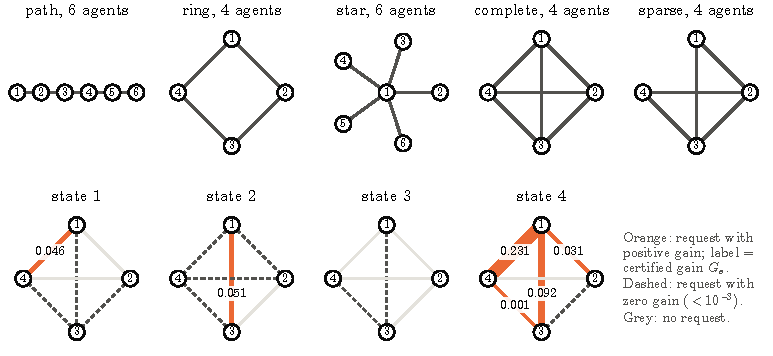
\includegraphics[width=\textwidth]{fig_network.pdf}
\caption{\emph{Top:} the five graph families. \emph{Bottom:} four of the 14 states of one catalog, with each request's certified gain. Edges that share an agent cannot be served in the same round.}
\label{fig:network}
\end{figure}

\paragraph{Data splits.} Request types and catalogs were generated with separate seeds for development (8 catalogs), validation (4), and test (4). The test catalogs include a graph larger than any seen in training (an eight-agent sparse graph) and a longer horizon ($H=24$), so they also test generalization. The environment also supports two imperfections found in real hardware, heralded loss and Werner noise.

%======================================================================
\section{Allocators}\label{sec:methods}
%======================================================================

We compare three groups of methods: learned allocators, simple baselines, and strong baselines.

\paragraph{Learned allocators.} DQN \citep{mnih2015human}, Double DQN \citep{vanhasselt2016deep}, PPO \citep{schulman2017proximal}, and recurrent PPO share a permutation-invariant encoder that scores each feasible matching from the per-edge gains, the remaining budget, and the remaining time (\cref{app:training}).

\paragraph{Simple baselines.} \emph{Greedy} always serves the highest-gain matching in the current round. \emph{Random} and \emph{static} are weaker and are included for reference.

\paragraph{Strong baselines.} We add two baselines that know how to pace a budget. Both were specified before they were run, and their parameters were chosen on validation catalogs only.

The \emph{bid-price rule} serves the best matching whose every edge has a positive gain of at least
\begin{equation}
  \theta_t=\begin{cases}0, & \alpha b_t\ge 2k_t,\\ Q_{\,1-\alpha b_t/(2k_t)}\bigl(\mathcal R_\omega\cup\mathcal O_t\bigr), & \text{otherwise,}\end{cases}
  \label{eq:bidprice}
\end{equation}
where $Q_q$ is the $q$-quantile of a weighted mixture of the gains seen in the training catalogs (total weight $\omega$) and the gains seen so far in the episode (weight one each). The term $\alpha b_t/(2k_t)$ is the share of the remaining request slots that the budget can afford, since at most two pairs are served per round. As a result, the threshold rises as pairs become scarce. For example, with $\alpha=0.75$, one pair left, and ten rounds to go, only roughly the top 4\% of gains are served. The rule has only two parameters, $(\alpha,\omega)$, and never sees the transition matrix $P$.

\emph{Certainty-equivalent DP (CE-DP)} plans exactly with the catalog's state table but replaces the true $P$ with a crude guess $\hat P$: stay in the current state with probability $\rho$ (the training average, \rhoFull) and otherwise move to any other state with equal probability. Logged episodes, if available, update the guess by counting transitions. It then solves
\begin{equation}
  V_k(s,b)=\max_{M\in\M(s,b)}\Bigl[\,G(s,M)+\textstyle\sum_{s'}\hat P(s,s')\,V_{k-1}\bigl(s',b-|M|\bigr)\Bigr],\qquad V_0\equiv0.
  \label{eq:bellman}
\end{equation}
CE-DP tells us how much is lost by not knowing how demand evolves. Since it sees the state table, which the learners and the bid-price rule do not, we treat it as a reference rather than a direct competitor. Its result is also not sensitive to the value of $\rho$: replacing $\rho$ with the true average stay probability changed CE-DP by at most \trMatchMaxDiff{} points (\cref{app:transitions}).

\paragraph{References.} \emph{Online DP} solves \cref{eq:bellman} with the true $P$. It is the best any real allocator can do, and we use it as 100\%. The \emph{future-clairvoyant} reference knows the whole state sequence in advance, which no real allocator can.

%======================================================================
\section{Experimental setup}\label{sec:protocol}
%======================================================================

Before any test file was read, the evaluation code first tuned the bid-price rule over \bpConfigs{} configurations on the four validation catalogs (500 sequences each) and saved the selected parameters, $\alpha=\cfAlpha$ and $\omega=\cfOmega$, to disk. It then trained 12 PPO and 12 DQN models on the 12 training catalogs and saved every checkpoint. The learners use the configurations selected on validation data in our learner-strength experiment (\cref{sec:followups}): width 64, learning rate $3\times10^{-3}$, 8{,}000 episodes for PPO with a calibrated value baseline, and 6{,}000 episodes for DQN. CE-DP uses $\rho=\cfRho$, the mean stay probability of the training catalogs. Only after that did the code read the test catalogs, re-certify their 16 request types (largest SDP gap \cfSdpMax), and evaluate every method once on the same 500 sequences per catalog. The whole run took \cfWallHours{} hours on four CPU cores. All of these steps, together with the hypotheses and decision rules below, were committed to a public repository before the run.

\paragraph{Statistical tests.} For each comparison we report the difference in mean surplus (e.g., PPO minus bid-price) with a 95\% confidence interval from 20{,}000 bootstrap resamples of the 12 training seeds \citep{efron1993introduction}. As decided before the test, a method is counted as better only if the whole interval lies on one side of zero.

%======================================================================
\section{Results and discussion}\label{sec:results}
%======================================================================

\subsection{Learners beat greedy}\label{sec:locked}

As shown in \cref{tab:main}, both learners clearly outperform greedy. PPO beats greedy by $\cfPpoMinusGreedy$ (95\% CI: $\cfPpoMinusGreedyLo$ to $\cfPpoMinusGreedyHi$), with all 12 seeds ahead, and DQN beats it by $\cfDqnMinusGreedy$. PPO reaches \cfFracPpo\% of the optimum and DQN \cfFracDqn\%, compared with only \cfFracGreedy\% for greedy. PPO also generalizes well, keeping at least \cfFracMinPpo\% on every catalog, including the larger graph and the longer horizon. PPO is also clearly better than DQN, by $\cfPpoMinusDqn$ (90\% CI: $\cfPpoMinusDqnLoNinety$ to $\cfPpoMinusDqnHiNinety$).

\begin{table}[t]
\centering
\caption{Results on the test catalogs: percentage of the online-DP optimum, with mean surplus in parentheses. Learned rows average 12 seeds. CE-DP can exceed 100\% slightly due to sampling noise.}
\label{tab:main}
\small
\setlength{\tabcolsep}{4pt}
\begin{tabular}{@{}lccccc@{}}
\toprule
Method & \shortstack{4-agent\\complete} & \shortstack{5-agent\\ring} & \shortstack{8-agent\\sparse} & \shortstack{6-agent path\\$H{=}24$} & Overall \\
\midrule
% Generated by make_tmlr_assets.py; do not edit.
Greedy & 52.3\,(0.310) & 41.2\,(0.245) & 39.5\,(0.544) & 41.8\,(0.388) & 42.6\,(0.372) \\
DQN & 93.9\,(0.557) & 81.4\,(0.484) & 70.3\,(0.969) & 76.5\,(0.710) & 77.9\,(0.680) \\
PPO & 86.8\,(0.515) & 95.2\,(0.566) & 94.0\,(1.294) & 94.5\,(0.877) & 93.1\,(0.813) \\
\midrule
\textbf{Bid-price} & \textbf{98.3}\,(0.583) & \textbf{98.1}\,(0.584) & \textbf{98.7}\,(1.360) & \textbf{98.6}\,(0.914) & \textbf{98.5}\,(0.860) \\
CE-DP, no data & 99.9\,(0.593) & 99.8\,(0.594) & 99.8\,(1.375) & 100.1\,(0.928) & 99.9\,(0.872) \\
\midrule
Online DP (true $P$) & 100.0\,(0.594) & 100.0\,(0.595) & 100.0\,(1.377) & 100.0\,(0.928) & 100.0\,(0.873) \\
Future-clairvoyant & 103.8\,(0.616) & 105.5\,(0.628) & 105.3\,(1.450) & 103.8\,(0.963) & 104.7\,(0.914) \\
\bottomrule

\end{tabular}
\end{table}

\subsection{A two-parameter rule beats every learned seed}\label{sec:strong}

However, the picture changes when the learners are compared with the bid-price rule. The rule reaches \cfFracBp\% of the optimum, and between \cfFracMinBp\% and \cfFracMaxBp\% on every catalog. PPO minus bid-price is $\cfPpoMinusBp$ (95\% CI: $\cfPpoMinusBpLo$ to $\cfPpoMinusBpHi$), so the rule is superior, and none of the 12 PPO seeds beats it; the best seed reaches \cfPpoBestSeedFrac\%. The gap is even larger for DQN ($\cfDqnMinusBp$, 95\% CI: $\cfDqnMinusBpLo$ to $\cfDqnMinusBpHi$). In other words, the rule closes \cfGapClosed\% of the gap that PPO leaves to the optimum. CE-DP, with no logged data at all, reaches \cfFracCe\% (\cref{fig:fraction}).

\begin{figure}[t]
\centering
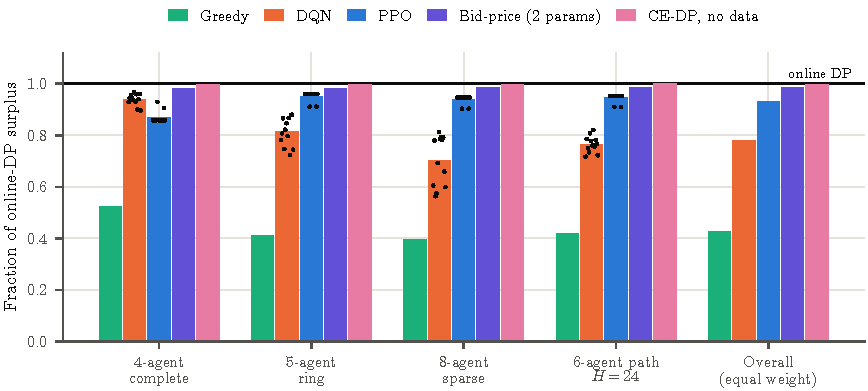
\includegraphics[width=\textwidth]{fig_confirm.pdf}
\caption{Percentage of the optimum on each test catalog. Dots are individual PPO and DQN seeds.}
\label{fig:fraction}
\end{figure}

\paragraph{Why the simple rules win.} Interestingly, CE-DP with a crude guess of $P$ performs almost as well as DP with the true $P$. This shows that knowing \emph{how} demand evolves is worth very little here, while knowing \emph{what} gains can appear and how many pairs remain is worth almost everything. Even perfect foresight adds only \cfForesight\% over online DP. The learners' shortfall therefore comes from budget pacing, which a simple quantile rule does better than a network trained from reward. This agrees with our development ablations, where removing the remaining-budget or remaining-time input hurt the learners the most (\cref{app:training}). The gap was also visible before the test: on validation catalogs, PPO reached \lsPPOFrac\% of the optimum against \lsRuleFrac\% for the rule.

\subsection{Follow-up experiments}\label{sec:followups}

We ran three follow-up experiments on development and validation data to check whether the result depends on our particular setup.

\paragraph{Were the learners under-tuned?} We widened the search grid (widths up to 256 and learning rates up to $10^{-2}$), trained about three times longer, calibrated PPO's value baseline, and used 6 seeds. PPO reached \lsPPOFrac\% of the optimum, still below the rule's \lsRuleFrac\% (difference $\lsPPOMinusRule$, 95\% CI: $\lsPPOLo$ to $\lsPPOHi$). PPO stopped improving after 4{,}000 episodes, and DQN became worse with longer training (\cref{app:strength}). The configurations selected here are the ones used in our main evaluation.

\paragraph{A harder variant designed for learning.} We built a variant with a hidden demand regime that only the history of states can reveal, which should favour learners with memory. Even so, the best learner (\rgBestName) reached \rgBestFrac\% of the optimum for that variant, against \rgRuleFrac\% for the rule. The gap was larger than the futility margin we had set in advance, so we stopped the study before its test (\cref{app:regime}).

\paragraph{Other dynamics.} We rebuilt the validation catalogs with six other transition matrices. The bid-price rule kept \trBpMin--\trBpMax\% of the optimum under all of them. CE-DP's crude guess held at \trCeOkMin\% or more, except when each state has an 80\%-likely successor (\trCeSucc\%), where ten logged episodes brought it back to \trCeSuccKten\% (\cref{app:transitions}). Pacing therefore generalizes across dynamics, while the dynamics only start to matter when the chain has strong structure.

%======================================================================
\section{Reproducibility}\label{sec:audit}
%======================================================================

Every test request type was re-certified at evaluation time, and the generator of the test split rejects any reuse of development or validation dynamics and requests. Every number in this paper is regenerated from the raw episode records by our build script, and matches the archived analysis to within $10^{-9}$. The code, data splits, records, and checkpoints are provided as anonymized supplementary material.

%======================================================================
\section{Discussion}\label{sec:discussion}
%======================================================================

In budgeted allocation, greedy is a weak baseline because it ignores the cost of spending a unit too early. If greedy had been our strongest baseline, PPO would have looked like a clear success. The bid-price rule shows that most of this gain can be obtained with two parameters and no training. We therefore recommend that future work on learned allocators include at least one pacing rule and one certainty-equivalent planner as baselines, and report every method as a percentage of an exact optimum, so that ``\cfFracPpo\% of optimal'' can be read against ``\cfFracBp\% from two parameters''.

Since this is a first study on BellRoute, there are several improvements that can be made in the future. Our catalogs are small (at most eight agents, 14 states, and four test catalogs) and come from a single generator, and we only tested MLP learners. \cfPpoSame{} of the 12 PPO seeds converged to the same test score, so PPO's confidence interval is narrow mainly because its seeds barely differ. The quantum model is also idealized, with single-hop links and no hardware. For example, larger networks, attention-based learners, and variants with unknown or changing state tables would be valuable directions for future study.

%======================================================================
\section{Conclusion}\label{sec:conclusion}
%======================================================================

In this paper, we introduced BellRoute, a benchmark for budgeted entanglement allocation with certified rewards and an exact optimum. Our results showed that deep RL allocators beat greedy by a wide margin and generalize to a larger graph and a longer horizon, but a two-parameter bid-price rule beats every learned model on test data seen only once. Three follow-up experiments did not change this result. Finally, the benchmark, code, and records are provided for future research.

\subsubsection*{Broader impact statement}
This work concerns resource allocation in simulated quantum networks and RL evaluation methodology. Its message, to compare learned controllers with strong classical rules, should reduce unnecessary complexity in deployed systems.

\subsubsection*{Use of AI tools}
The experiment code, analysis, audit, and drafts of this manuscript were produced with AI coding assistants under the authors' direction within a recorded, version-controlled protocol. The authors reviewed the work and take responsibility for its content.

\bibliography{references}
\bibliographystyle{tmlr}

\appendix

\section{A worked request type and all catalogs}\label{app:xor}

\Cref{tab:xor} shows one development request type. The best classical plan, $a=(0,0,1)$ and $b=(0,1,1)$, wins seven of the nine question pairs, giving $V_C=\xorClassical$. With a Bell pair the players win $V_Q=\xorBell$: they win no pair with certainty, but they win the heavy pair $(\xorRecX,\xorRecY)$, which the classical plan always loses, with probability \xorRecQ.

\begin{table}[H]
\centering\small
\caption{Request type \texttt{qip-development-type-000}, one row per question pair.}
\label{tab:xor}
% Generated by make_tmlr_assets.py; do not edit.
\begin{tabular}{c|ccc}
$x\backslash y$ & 0 & 1 & 2 \\
\hline
0 & 0\,/\,1 & 1\,/\,2 & 0\,/\,1$^{\times}$ \\
1 & 0\,/\,3 & 1\,/\,3 & 1\,/\,4 \\
2 & 0\,/\,4$^{\times}$ & 0\,/\,4 & 0\,/\,3 \\
\end{tabular}

\end{table}

\begin{table}[H]
\centering\small
\caption{All catalogs. ``Stay'' and ``Next'' are mean probabilities of staying in the same state and of moving to the next state in the generator's cycle. }
% Generated by make_tmlr_assets.py; do not edit.
\begin{tabular}{@{}llrrrrrrr@{}}
\toprule
Split & Topology & Agents & Edges & $H$ & $B$ & Requests/state & Stay & Next \\
\midrule
Dev. & path & 3 & 2 & 8 & 2 & 2.0 & 0.36 & 0.15 \\
 & ring & 3 & 3 & 10 & 4 & 2.4 & 0.31 & 0.14 \\
 & complete & 4 & 6 & 10 & 6 & 4.4 & 0.33 & 0.17 \\
 & path & 4 & 3 & 16 & 6 & 2.4 & 0.37 & 0.16 \\
 & ring & 4 & 4 & 10 & 4 & 3.1 & 0.37 & 0.15 \\
 & star & 4 & 3 & 12 & 4 & 2.3 & 0.36 & 0.14 \\
 & path & 6 & 5 & 16 & 6 & 3.5 & 0.34 & 0.13 \\
 & star & 6 & 5 & 10 & 4 & 3.8 & 0.34 & 0.14 \\
\midrule
Val. & ring & 3 & 3 & 8 & 2 & 2.4 & 0.31 & 0.14 \\
 & sparse & 4 & 5 & 12 & 4 & 3.7 & 0.35 & 0.15 \\
 & path & 6 & 5 & 16 & 6 & 2.9 & 0.34 & 0.14 \\
 & star & 6 & 5 & 10 & 4 & 3.6 & 0.37 & 0.14 \\
\midrule
Test & complete & 4 & 6 & 10 & 6 & 3.8 & 0.34 & 0.16 \\
 & ring & 5 & 5 & 16 & 6 & 3.6 & 0.36 & 0.16 \\
 & sparse & 8 & 11 & 24 & 10 & 5.5 & 0.36 & 0.15 \\
 & path & 6 & 5 & 24 & 8 & 3.5 & 0.35 & 0.16 \\
\bottomrule
\end{tabular}

\end{table}

\section{Learner training}\label{app:training}

Learners use Adam \citep{kingma2015adam}, gradient clipping at 5, and reward scale 10. DQN uses a 20{,}000-transition replay buffer, minibatches of 64, and target copies every 200 updates; PPO uses 16-episode rollouts and 4 epochs of the clipped objective. The configurations used in the main evaluation were selected in the learner-strength check (\cref{app:strength}). In Double DQN ablations, removing the remaining-budget input cost \ablDropNoBudget\% of validation surplus and removing the remaining-time input cost \ablDropNoHorizon\%.

\section{Learner-strength check}\label{app:strength}

Configurations were selected on 200 validation sequences per catalog using 2 seeds each, the selected one was retrained with 4 more seeds, and all methods were compared on 500 fresh sequences per catalog. The registered decision was \texttt{\lsDecision}.

\begin{table}[H]
\centering\small
\caption{Learner-strength check on validation catalogs. The comparison column gives the percentage of the online-DP optimum (\lsOnlineMean), with the mean surplus in parentheses.}
% Generated by make_tmlr_assets.py; do not edit.
\begin{tabular}{llrrr}
\toprule
Method & Configuration & Seeds & Selection mean & Comparison: \% of online DP (mean) \\
\midrule
PPO & h64-lr1e-3 & 2 & 0.3226 & 85.7\,(0.3169) \\
PPO & h64-lr3e-3 (selected) & 6 & 0.3343 & 88.2\,(0.3260) \\
PPO & h64-lr1e-2 & 2 & 0.3391 & 89.3\,(0.3302) \\
PPO & h256-lr1e-3 & 2 & 0.3383 & 89.0\,(0.3292) \\
PPO & h256-lr3e-3 & 2 & 0.3367 & 88.7\,(0.3280) \\
PPO & h256-lr1e-2 & 2 & 0.3367 & 88.7\,(0.3280) \\
\midrule
DQN & h64-lr1e-3 & 2 & 0.2982 & 79.9\,(0.2955) \\
DQN & h64-lr3e-3 (selected) & 6 & 0.3043 & 81.4\,(0.3011) \\
DQN & h64-lr1e-2 & 2 & 0.3066 & 81.6\,(0.3017) \\
DQN & h256-lr1e-3 & 2 & 0.2956 & 79.7\,(0.2945) \\
DQN & h256-lr3e-3 & 2 & 0.2985 & 79.7\,(0.2945) \\
DQN & h256-lr1e-2 & 2 & 0.3130 & 83.1\,(0.3071) \\
\midrule
Bid-price & $\alpha{=}0.75$, $\omega{=}320$ & -- & -- & 96.7\,(0.3576) \\
\bottomrule
\end{tabular}

\end{table}

\section{The hidden-regime variant}\label{app:regime}

Each episode secretly draws a ``rich'' or ``lean'' demand regime that tilts the transition matrix, and the current state alone does not reveal it. The optimum is a DP over the state and the posterior probability of each regime (a belief-state DP); knowing the regime outright would add only \hrRegimeOracle\% to it. DQN, PPO, and recurrent PPO were tuned equally (6 configurations, 3 seeds, 2{,}000 episodes each) and selected on validation catalogs, where the bid-price rule was also tuned. The registered futility rule stopped the study if the best learner trailed the rule on validation by more than 5\% of the optimum (\rgMargin); the gap was \rgGap.

\section{Robustness to the transition matrix}\label{app:transitions}

Each validation catalog was rebuilt under each transition matrix, keeping its state table. ``Stay $s$'' sets the self-loop probability to $s$; ``successor $w$'' sends each state to a fixed other state with probability $w$; ``rare jackpot'' makes the most valuable state rare but persistent. The bid-price rule was retuned for each matrix on separate tuning sequences.

\begin{table}[H]
\centering\small
\caption{Percentage of the online-DP optimum on the validation catalogs under rebuilt transition matrices.}
% Generated by make_tmlr_assets.py; do not edit.
\begin{tabular}{lrrrrrrr}
\toprule
& & & \multicolumn{2}{c}{Bid-price} & \multicolumn{3}{c}{CE-DP} \\ \cmidrule(lr){4-5}\cmidrule(l){6-8}
Transition matrix & Stay & Greedy & frozen & retuned & default & $K{=}10$ & $K{=}100$ \\
\midrule
as generated & 0.34 & 58.5 & 96.8 & 96.8 & 99.8 & 99.7 & 100.0 \\
stay 0.05 & 0.05 & 55.9 & 97.2 & 97.6 & 99.6 & 99.6 & 99.9 \\
stay 0.7 & 0.70 & 64.2 & 96.0 & 96.4 & 99.4 & 99.4 & 99.8 \\
stay 0.9 & 0.90 & 71.5 & 95.8 & 96.4 & 98.6 & 99.2 & 99.6 \\
successor 0.5 & 0.17 & 58.7 & 95.8 & 96.4 & 98.9 & 99.7 & 100.0 \\
successor 0.8 & 0.07 & 59.3 & 94.0 & 94.9 & 96.5 & 98.9 & 99.9 \\
rare jackpot & 0.37 & 63.0 & 95.7 & 97.8 & 99.3 & 99.5 & 99.9 \\
\bottomrule
\end{tabular}

\end{table}

\end{document}
